\section{Feature Extraction }
In this section, we introduce the detailed approaches how we uniquely represent the Android apps. The CFG(Control Flow Graph) is the common feature used in bug search. Moreover, different from other attributes on the basic blocks, such as I/O pairs and statics features \cite{23}\cite{45(SGbBSfFI)}, are more accuracy matching. Following  the idea of the original CFG extraction, this paper utilizes the control flow graph with different basic-block level attributes about five features based, it called as the 5UD-CFG. We also prove the monotonicity of the feature of the 5UD-CFG. A feature of 5UD-CFG represents a CFG.

\subsection{Disassembly of Android Application and CFG extraction}
In our system, the preprocessing of an application consists of disassembling the application and extracting opcode sequences. A code file is a dex file that can be transformed into smali files, where each smali file represents a single class and contains the methods of such a class. Each method contains instructions and each instruction consists of a single opcode and multiple operands.  

After preparation, including downloading all the apps from multiple markets or malware database and extracting methods from the apps, we encode a projection form of CFG to get the unique feature of the function of an apk.

CFG is the control flow graph of a method. Each node in a CFG corresponds to a basic block in the method. A basic block is a straight-line piece of code with one entry point and one exit point. Jump targets start a block, and jump end a block. Directed edges are used to represent jumps in the control flow.

\subsection{5UD-CFG}
In this paper, we extract the unique property of CFG by a number list, which is proved monotonically represent its corresponding CFG. Android apps are written in JAVA, which is a kind of structured programming. Sequence, branch and circulation are three basic structures to encode a CFG to 5UD-CFG.

\textbf{Definition 1.} (5UD-CFG) The control flow graph with five unique feature, or 5UD-CFG in short, is a directed graph $G=<V,E>$, where $V$ is a set of basic block in a function;$E \subseteq V \times V$ is a set of edges representing the connections between these basic blocks. Each node in $V$ has a unique coordinate. The coordinate of a node is a vector $<n, s, i, o, l>$. $n$ is the sequence number of a node in the CFG, $s$ is the number of opcodes of a basic block, the $i$ is the number of input edges of the node (the basic block), $o$ is the number of outgoing edges of the node. $l$ is the number of the loop of a node.

Fig. 1 shows a real CFG of a function in a class. A node represents a basic block, and a edge represents a call link between two basic block. A basic block is a set of opcodes. The outgoing edges of a node $A$ represents the basic block $A$ is called by other basic block. The input edges of a node $A$ represents the basic block $A$ calls other basic blocks. 

\begin{figure}[hbt]
  \center{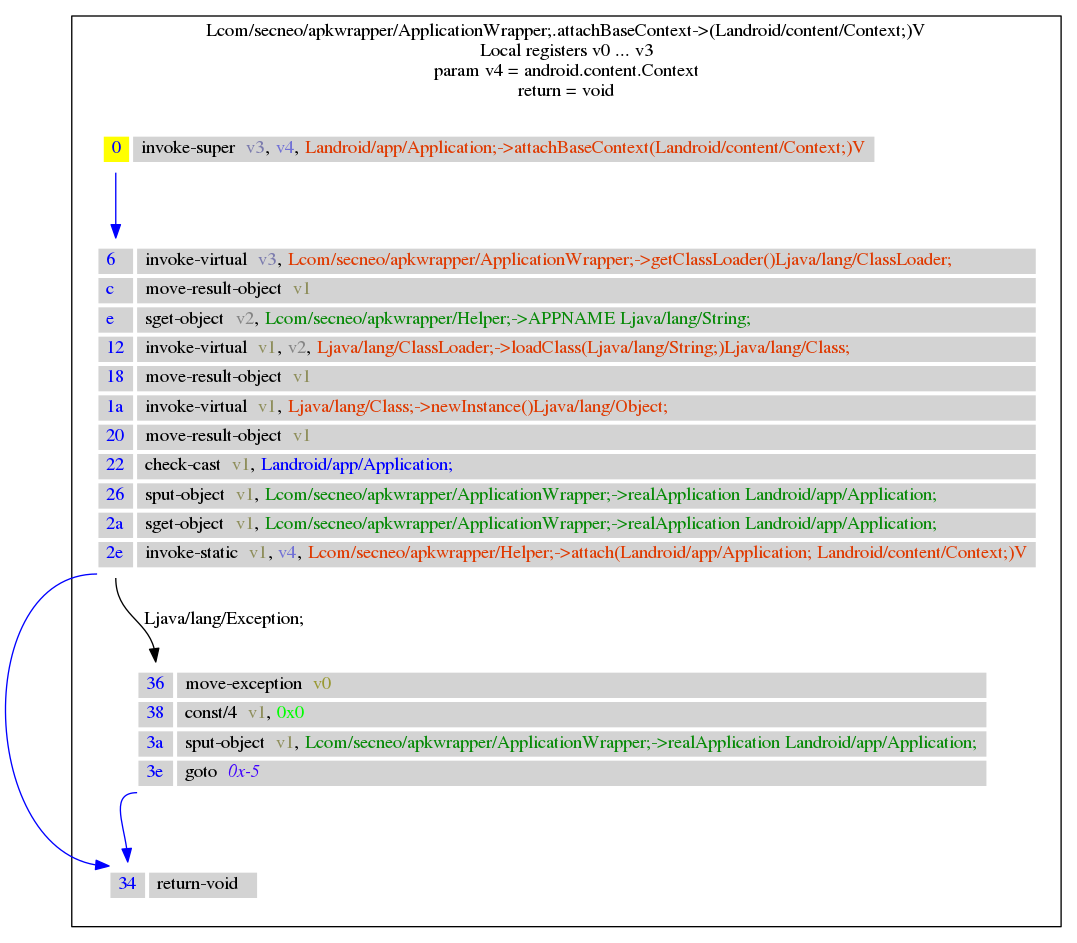
\includegraphics[width=8cm] {cfgexample.png}}
  \caption{\label{1} My figure.  An example of a method cfg in a real apk}
\end{figure}

There is a unique mapping between a CFG and a 5UD-CFG. The same node in a CFG has the same sequence number, which is decided by the order in which it executes. The entry node is with the number 1. The sequence number list of all nodes shows the result of the breadth first search in the CFG. For example, as shown in the Fig.1 and the Fig. 2, it is the CFG and the 5UD-CFG of a real method in a apk. Node $A$ in the CFG is the starting node with the sequence number 1. The sequence number of $B$ is 2, and so on $C$ is 3, $D$ is 4, and $E$ is 5. The loop of a node shows there is a directed circle from the node back to the node. The number of the loop of the $A$ is 0, $B$ is 1, $C$ is 1, $D$ is 0, and $E$ is 0. Other features are shown in the Fig. 2(b).

A 5UD-CFG can be viewed as a set of nodes connected by edges. We need to define the node weight of each node (basic block). The node weight of each node is used to combine all node to represent the CFG. We define the feature of a 5UD-CFG based on the 3D-CFG \cite{chenkai}.

\textbf{Definition 2.} A feature of a 5UD-CFG is a vector $<f_n, f_s, f_i, f_o, f_l>. f_n=\frac{\sum_{e(j,k)\in 5UD-CFG}(\omega_jn_j+\omega_kn_k)}{\omega}, \\ f_s=\frac{\sum_{e(j,k)\in 5UD-CFG}(\omega_js_j+\omega_ks_k)}{\omega}, \\ f_i=\frac{\sum_{e(j,k)\in 5UD-CFG}(\omega_ji_j+\omega_ki_k)}{\omega},\\ f_o=\frac{\sum_{e(j,k)\in 5UD-CFG}(\omega_jo_j+\omega_ko_k)}{\omega}, \\f_l=\frac{\sum_{e(j,k)\in 5UD-CFG}(\omega_jl_j+\omega_kl_k)}{\omega} and \\ \omega=\sum_{e(j,k)\in 5UD-CFG}(\omega_j+\omega_k)$.
 
In Definition 2, $e(j, k)$ is an edge in CFG. This edge connects two nodes $j$ and $k$. The key factor of the feature of a 5UD-CFG is the node weight $\omega$. We define the $\omega$ as follows:

\textbf{Definition 3.} $\omega_j$ is the number of other nodes that node $j$ are called as the father node or the grandfather node in a CFG. It is shown in a figure that node $j$ is link with how many other nodes as the directed outgoing paths. $\omega$ is the sum of $\omega_j$ for all nodes in a CFG.

we give an example to show how to calculate the $\omega_j$. Node $A$ with the first sequence number is called by the node $B$ and the node $C$ directly. Node $C$ is called by the node $D$ directly, and node $D$ is called by the node $E$ directly. This outgoing degree of node $A$ is $A_{\searrow B}^{\nearrow C \longrightarrow D \longrightarrow E}$. $A$ is related with $B$, $C$, $D$ and $E$, so the $\omega_A =4, \omega_B=0, \omega_C=2, \omega_D=1, \omega_E=0.$ The result of node $A$ will be passed to node $B$ and node $C$. This process will also influence the node $D$ and $E$ by influencing the node $C$. 

The node weight $\omega_j$ is unique when the CFG is determined. As the view of the Definition 2, the $\omega_j$ is related with the $\sum_{e(j,k)\in 5UD-CFG}$.  We can see $\omega~e$, $e$ is the edge in the CFG. The different CFG has the different node weight sequence $\omega_j, j={1,2,3,...,n} and \omega_j<n-1$.

As shown in the Fig. 2, we calculate the feature of a 5UD-CFG as follows:
\begin{eqnarray*}
	\begin{cases}
		f_n=\frac{1\times 2\times 4+ 2\times 1\times 0+3\times 2\times2+ 4\times 2\times 1 +5\times 1 \times 0}{4+0+2+1+0}=4\\
		f_s=\frac{1\times 2\times 4+ 7\times 1\times 0+4\times 2\times2+ 4\times 2\times 1 +1\times 1 \times 0}{4+0+2+1+0}=4.571\\
		f_i=\frac{0\times 2\times 4+ 1\times 1\times 0+1\times 2\times2+ 1\times 2\times 1 +1\times 1 \times 0}{4+0+2+1+0}=0.857\\
		f_o=\frac{0\times 2\times 4+ 2\times 1\times 0+1\times 2\times2+ 1\times 2\times 1 +0\times 1 \times 0}{4+0+2+1+0}=0.857\\
		f_l=\frac{0\times 2\times 4+ 0\times 1\times 0+0\times 2\times2+ 0\times 2\times 1 +0\times 1 \times 0}{4+0+2+1+0}=0\\
		\omega=4+0+2+1+0=7.
	\end{cases}
\end{eqnarray*}

\begin{figure}[hbt]
  \center{\includegraphics[width=8cm] {cfg.eps}}
  \caption{\label{1}  An example of real CFG}
\end{figure}

\begin{figure}[hbt]
  \center{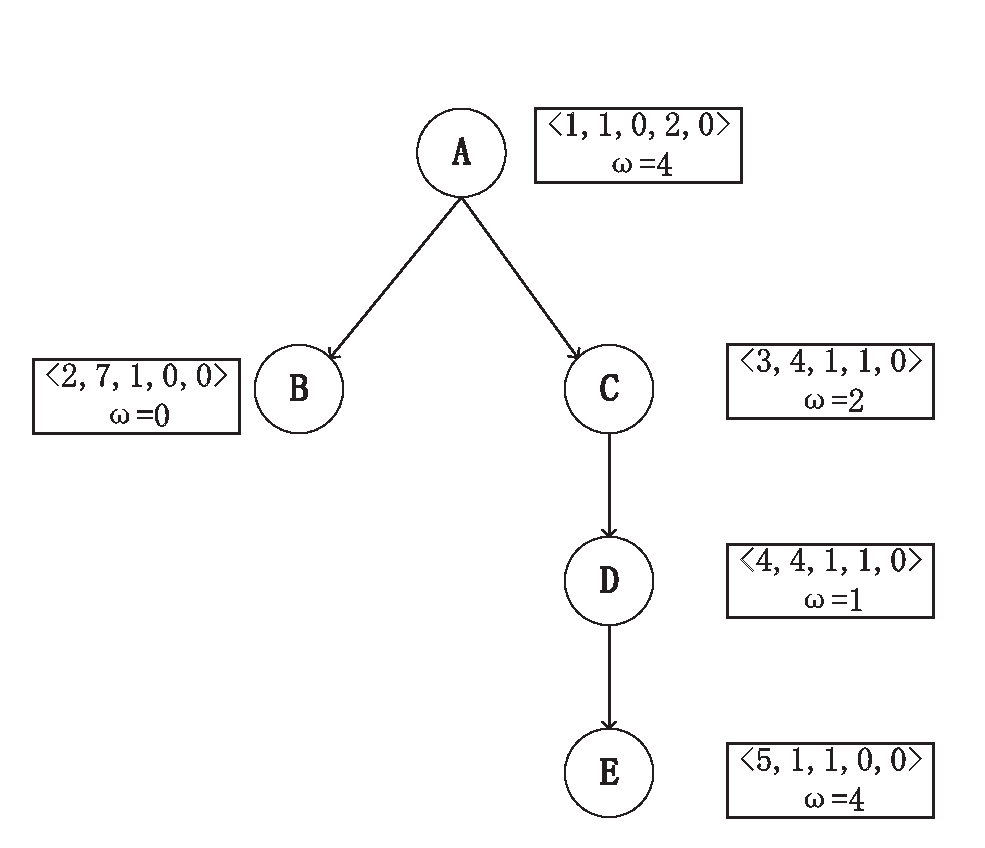
\includegraphics[width=8cm] {feature.eps}}
  \caption{\label{1}  An example of feature of 5UD-CFG}
\end{figure}

\subsection{Monotonicity of feature of 5UD-CFG} 
It is important to prove the monotonicity of the feature of the 5UD-CFG. The monotonicity shows the different CFGs have the different feature, at the same time, the same CFG has the same feature.  
\begin{proof}
	We use a expression to show the relationship between the edge set $E$ and the node weight set $W$, $W=f(E)$, the $f()$ is not a continuous function, is a discrete functions. If the $E_{CFG_j}=E_{CFG_k}$, the $W_{CFG_j} = W_{CFG_k}$. Exchanging condition and conclusion, it is also established. If the $W_{CFG_j} = W_{CFG_k}$, the $E_{CFG_j}=E_{CFG_k}$.
	
	Based on the Definition 3, the element in $W$, $\omega_j$ is calculated as follows:
	\begin{equation}
			\omega_j=\sum_{k\in j_o}(\omega_k +1),
	\end{equation}
	where the $j_o$ is the node-set of the outgoing degree of the node $j$. In a certain CFG, the $\omega_j$ of each node is determined by the iteration method. Therefore the $\omega_j~e_j$,is written by the $\omega_j=f(e_j)$. When the CFG is determined, the directed edges set $E$ of CFG is determined, therefore the node weight $\omega_j$ of each node is determined.
	
	Based on the Definition 2, we have
	\begin{equation*}
		\begin{split}
			& f_n=\frac{\sum_{j=1}^n \omega_j j e_j}{\omega}=\frac{\sum_{j=1}^n f(e_j) j e_j}{\omega}.\\
			& f_s=\frac{\sum_{j=1}^n \omega_j s_j e_j}{\omega}=\frac{\sum_{j=1}^n f(e_j) s_j e_j}{\omega}.\\
			& f_i=\frac{\sum_{j=1}^n \omega_j i_j e_j}{\omega}=\frac{\sum_{j=1}^n f(e_j) i_j e_j}{\omega}.\\
			& f_o=\frac{\sum_{j=1}^n \omega_j o_j e_j}{\omega}=\frac{\sum_{j=1}^n f(e_j) o_j e_j}{\omega}.\\
			& f_l=\frac{\sum_{j=1}^n \omega_j l_j e_j}{\omega}=\frac{\sum_{j=1}^n f(e_j) l_j e_j}{\omega}.\\
		\end{split}
	\end{equation*}
	
	We use reduction to absurdity to proof the monotonicity of feature of the 5UD-CFG. Assuming that there are two different CFGs' features are the same, therefore the $\omega$ is the same. And the following equations are the same.
	\begin{eqnarray*}
		\begin{cases}
			\sum_{j=1}^{n_1} f_1(e_{1j}) j e_{1j}=\sum_{j=1}^{n_2} f_2(e_{2j}) j e_{2j}\\	
			\sum_{j=1}^{n_1} f_1(e_{1j}) s_{1j} e_{1j}=\sum_{j=1}^{n_2} f_2(e_{2j}) s_{2j} e_{2j}\\
			\sum_{j=1}^{n_1} f_1(e_{1j}) i_{1j} e_{1j}=\sum_{j=1}^{n_2} f_2(e_{2j}) i_{2j} e_{2j}\\
			\sum_{j=1}^{n_1} f_1(e_{1j}) o_{1j} e_{1j}=\sum_{j=1}^{n_2} f_2(e_{2j}) o_{2j} e_{2j}\\
			\sum_{j=1}^{n_1} f_1(e_{1j}) l_{1j} e_{1j}=\sum_{j=1}^{n_2} f_2(e_{2j}) l_{2j} e_{2j}\\
			\sum_{j=1}^{n_1} f_1(e_{1j})=\sum_{j=1}^{n_2} f_2(e_{2j}).
		\end{cases}
	\end{eqnarray*}
	
	Before proving, we cite a existing lemma in the graph theory \cite{Feng} to prove the monotonicity of the feature of the 5UD-CFG.
	
	\begin{lemma}
		If the directed graph $G$ and the directed graph $G'$ are isomorphic,the input degree set $I$ and outgoing degree set $O$ of $G$, and the input degree set $I'$ and outgoing degree set $O'$ of $G'$ respectively are the same, $I=I'$ and $O=O'$. At the same time, the inverse is also true. 
	\end{lemma}
	
	We know the input degree set, the output degree set and the set of the number of loops in CFG $i, o, l$ is also determined by the edge set $E$. Based on the lemma 1, the edge set $E$ is also determined when the $i, o, l$ sets are determined. That is, if the input degree set of all nodes $i_{CFG_j} = i_{CFG_k}$ in a CFG, the $E_{CFG_j} = E_{CFG_k}$, if the outgoing degree set of all nodes $o_{CFG_j} =o_{CFG_k}$, the $E_{CFG_j}= E_{CFG_k}$ and if the $l_{CFG_j} = l_{CFG_k}$, the $E_{CFG_j}= E_{CFG_k}$. At the same time,  we know if the $W_{CFG_j} = W_{CFG_k}$, the $E_{CFG_j}= E_{CFG_k}$. Therefore, only if $n_1=n_2, e_{1j}=e_{2j}, f_1(e_{1j})=f_2(e_{2j}), j={1,2,...,n_1(n_2)}$, the equalities (1) are established.  
	Therefore, these two different CFGs actually are a same CFG. It does not exist two different CFGs have the same feature based on the proposed feature of 5UD-CFG.
\end{proof}

According to the above proof, we can know the proposed feature of 5UD-CFG is discrete monotonous. The different CFG has the different feature and the same CFG has the same feature. 
